This section will discuss the implementation, integration and testing of the SafeStreet application. The section aims to prevent any setbacks entailing changes on the project once started its development and do multiple tasks twice. First of all, it is important to divide the project into smaller components in order to have more concrete goals that help keep the developers’ motivation high and make a straightforward development of the project. Therefore, we will divide the project in dfferent components, starting from the ones that are responsible of the basic features and going on until the end, where we will develop the most specific ones. It is not a new method, because it has been studied during this course and it is referred to as ‘bottom-up’ strategy. This method will help providing a better integration of the project tier-by-tier and make different tests of the behaviour of the application before it ends. The System can be divided into three main parts as following:
\begin{itemize}
    \item \textbf{Frontend components:} contains the Mobile App.
    \item \textbf{Backend components:} contains the application server with all its components and the DBMS.
    \item \textbf{External components:} contains all the external components, such as the ALPR, to extract the license plate from a photo, and so on.
\end{itemize}
 It should be noted that the external systems’ components need not to be implemented and tested just because they are external and they can be considered reliable.
Going back to our project, we will divide the Mobile App component to three main entities, corresponding to USer, Violation and Ticket.
The services that have to be created for each entity are:
\begin{itemize}
\item{} \textit{User}: Sign-UP, Login
\item{} \textit{Violation}: Report Violation, Take Picture, Fill Form, Violation Info, List Vehicles, Street Heatmap, Mine information.
\item{} \textit{Ticket}: Ticket Approval, Statistics, Ticket offenders, Trends.
\end{itemize}

\begin{sidewaysfigure}
\centering
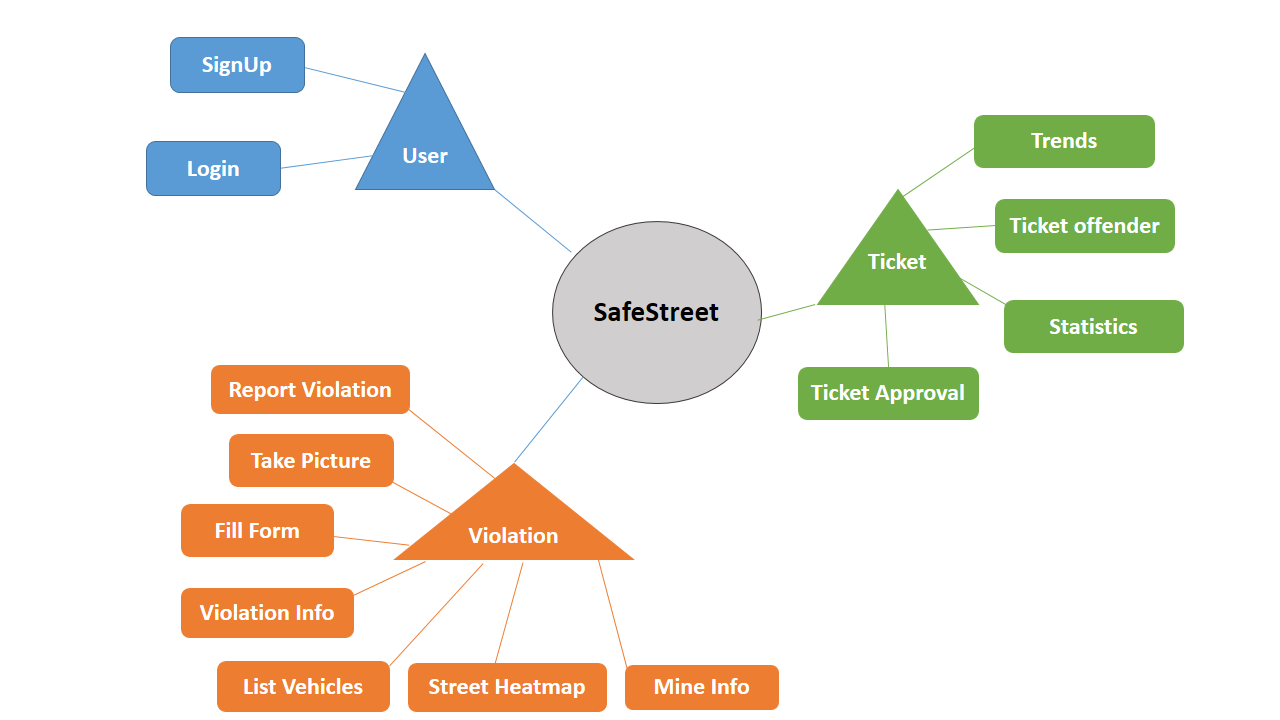
\includegraphics[width=\textwidth]{Images/ImplemetationandTest.png}
\caption{\label{fig:Test} A general overview of the service implementation}
\end{sidewaysfigure}

In figure \ref{fig:Test}, the overall process structure of the implementation has been shown. First, the blue part, will be implemented and tested. After the blue part works efficiently, the orange part, services related to report a violation, will be implemented and tested. Finally, if the blue and orange part will work efficiently, the final green part, Ticket, will be implemented and tested. During the implementation and testing process, we will make the component integration once we have finished each tier and tested each isolated component, meaning we will mix the different phases and try to detect possible defaults in our design.

As mentioned in \ref{fig:Test}, we will start with developing the User component. The Sign-Up and Login components are clearly an entry condition for the right functioning of the system, but they are not the main features and they are not very compicated. These two components can be implemented and tested at any order. After Implemeting and testing User component, we will continue with the next part of the implementation of the software which is Violation component. We will integrate all the services and test whether the whole Violation component will work as it is expected. If the result is positive, we will continue with the next last of the implementation of the software. If the result is negative, we should study if something is wrong in our code or if we should make any changes in the project development.

\subsection{Sequence of component integration}
The diagrams below describe the sequence of the component implementation, integration and testing of the system. The arrows starts from the component which uses the other one.

\paragraph{Integration of the all internal components of the application server}
Firstly all the components will be implemented and tested with unit tests. Then the integration process will proceed in the following order and the integration is tested as well.

\begin{figure}[H]
\centering
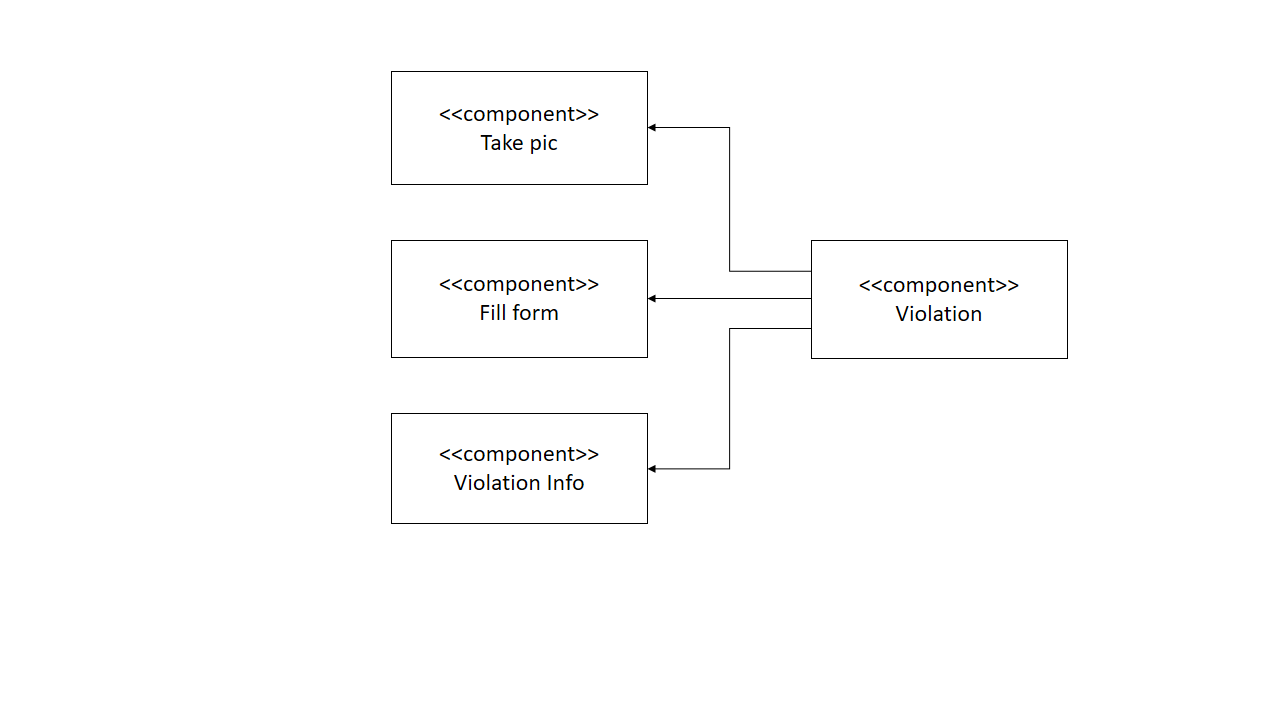
\includegraphics[width=\textwidth]{Images/reportviolationintegration.png}
\caption{\label{fig:reportviolationintegration} report violation integration}
\end{figure}

\begin{figure}[H]
\centering
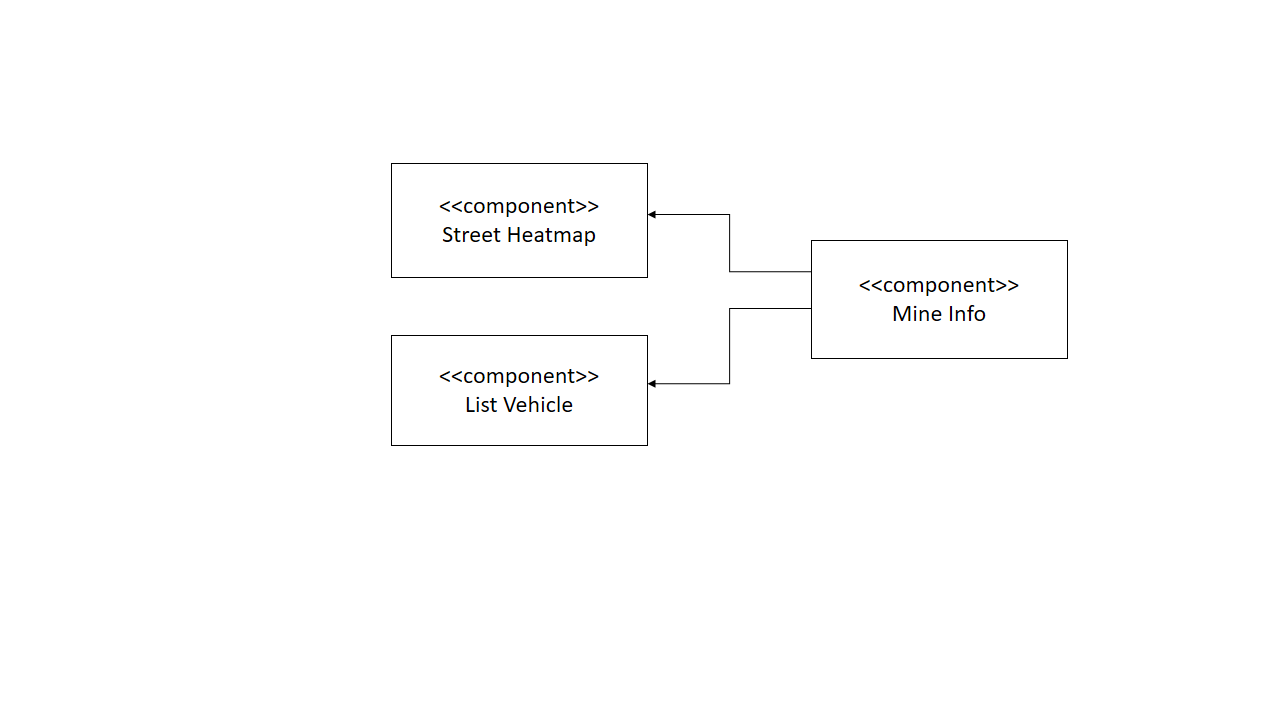
\includegraphics[width=\textwidth]{Images/MineInfoIntegration.png}
\caption{\label{fig:MineInfoIntegration} Mine Information integration}
\end{figure}
